\textbf{\textit{“Good architecture makes the system easy to understand, easy to develop, easy to maintain, and easy to deploy. The ultimate goal is to minimize the lifetime cost of the system and to maximize programmer productivity.” - Robert C. Martin}} \cite{10}

The previous section explained that software systems are not static environments. They grow, change, and get updated based on the new requirements. During this change, new additions are made in forms of components, methods, modules. As the system grows, the interactions between these different system elements also get more complicated and all together lead to complexity in software systems. In order to be able to develop reliable software systems that can overcome this complexity, programmers must implement software systems in a generalized fashion. Software systems that are written in such fashion can be considered reliably usable, maintainable, testable, and extendable \cite{15}. 

At that stage, the question is, what would be the so-called generalized fashion from the software engineering perspective. A couple of decades ago, software engineers and researchers started paying more attention to this topic and started studies to find an answer to this question. These studies were intended to find solutions for the problems emerging while developing large scale software systems. The focus area of these studies started as software design and eventually evolved into software architecture \cite{24}. The answer to the above question today is software architecture. Martin Fowler defines the meaning of the architecture in the software industry as "the shared understanding that the expert developers have of the system design" \cite{16}. Technically speaking, software architecture is "the set of significant decisions about the organization of a software system, the selection of structural elements and their interfaces by which the system is composed, together with their behavior as specified in the collaborations among those elements, the composition of these elements into progressively larger subsystems, and the architectural style that guides this organization -- these elements and their interfaces, their collaborations, and their composition" \cite{17}. 

Good architecture facilitates the satisfaction of requirements for software systems as well as providing better performance and more reliability. Today the impact of software architecture on the success of software systems is quite high. Selecting the right architecture for a software system is a critical success factor for system design and development. As Brian Foote quotes, "if you think good architecture is expensive, try bad architecture"\cite{10}. Also, software architecture has a central role between software implementation and requirements. The role of software architecture in software development can be elaborated under the six major aspects. Those aspects can be listed as follows \cite{25}:
\begin{itemize}
    \item \textbf{Understanding:} Good architectural design simplifies the understanding of systems, in the context of what the system does and how it does as well as facilitating the understanding of the systems’ high-level design. Thus good architecture improves the readability of software systems.
    \item \textbf{Reuse:} Good software architecture facilitates and increases the code reuse between the components.
    \item \textbf{Construction:} Software architecture provides a good outline of the software system in the form of layers and abstractions. The outline describes the components of the system and dependencies between those components.
    \item \textbf{Evolution:} Software architecture can point out the dimensions which a software system might evolve to. Therefore software architecture helps software teams to understand the consequences of changes more accurately. Moreover, software architecture describes how the concerns of the software systems are separated and it determines the boundaries of interactions between those concerns. 
    \item \textbf{Analysis:} A well-applied software architecture enables analyzing the system consistency, compliance with restrictions imposed by the architecture, and compliance with the quality attributes.
    \item \textbf{Management:} Assessment of software architecture facilitates understanding of risks, requirements, and implementation strategies.
\end{itemize}
When contemplating the importance of software architecture for Android application development, of course, there is no difference. When the fast update rate of Android applications, frequent requirement changes of Android projects, and the complex issues and restrictions that arise from the nature of Android are taken into consideration, the significance of software architecture selection when developing Android applications becomes even more prominent. However, this area has been problematic for Android application development and Android developers from the beginning.

During the early days of Android development, Android developers tended to use "god activities". God activities were activities where developers place all kinds of code including user interface, presentation logic, business logic, and so on. This unstructured way of a software development approach that does not follow any architectural or design pattern is called "anti-pattern". Back then, Android applications were relatively smaller and less complex. Ever since the Android applications started becoming more and more complex these god activities became a black hole for Android developers because they were hard to read, understand, test, and maintain. Android developers were quick to recognize these problems and needs and had no trouble finding solutions on how to develop Android applications in a more organized way. In order to solve this god activity and such an anti-pattern problem and improve the maintainability of Android applications, Android developers started applying well-known and widely used architectural and design patterns in GUI-heavy applications to Android application development \cite{19}. With improvements and advancements in hardware and software and growing demand for the user and business needs, the requirement for developing organized and maintainable Android applications has had a great extent \cite{18}.

Today, though the use of architectural patterns and design patterns in Android application development does not seem to be a requirement, it is actually of a de-facto must. Developing an Android application without applying an architectural pattern would be a bad decision because complex applications that do not follow any architectural pattern are expected to end up with serious maintainability issues. Also, surviving in such a competitive market is heavily dependent on developing a well-architected Android application that has a high level of maintainability. While developing Android applications, the expectation in terms of software architecture is to apply the SOLID principles and separation of concerns in a healthy way and to have high maintainability. On the other hand, there is no fixed solution for that problem that Android demands from developers to meet its applications and there are a variety of options. So, the right way to architect Android apps still remains in discussion with clashing standpoints which are generally affected by technological hypes \cite{14}.

Importance of the software architecture in terms of software systems and especially Android applications was explained above. At this point, it will be of utmost importance to emphasize the relationship between architectural choice and maintainability, as the main subject of the study is the improvement of the maintainability of Android applications. Can it be claimed that maintainability is the most crucial quality requirement when developing Android applications when it comes to architectural selection? With many options available for architecting Android applications, what is the top quality requirement that an Android application architecture should provide in order to overcome the complexities? As this study has emphasized continuously since the beginning, the answer to these questions is maintainability. A related study had conducted a questionnaire between Android practitioners and researched other related academic papers and results had revealed that the top quality requirement for architecting Android applications is maintainability \cite{14}.
\begin{figure}[ht!]
    \centering
    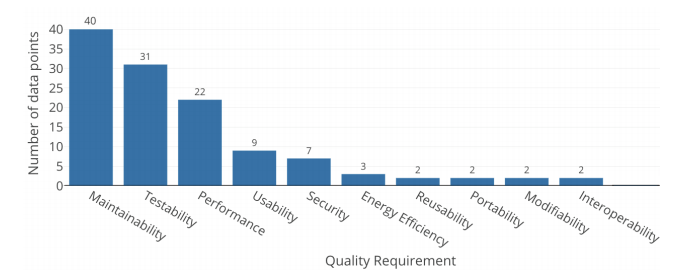
\includegraphics[scale=0.6]{figures/quality_req.png}
    \caption{Quality requirement rankings for architecting Android apps \protect\cite{14}}
    \label{fig:arch_quality_req_ranking}
\end{figure}

It is proven that maintainability and selection of architectural patterns when developing Android applications are directly in correlation. In addition, it can be said that other quality requirements presented in the figure above, apart from maintainability, directly affect maintainability itself. In particular, quality requirements such as modifiability, testability and reusability will increase as the maintainability increases, or vice versa. As a consequence, the impact of the architectural pattern on the maintainability of Android applications is one of the top aspects that should be considered when making the decision of the architectural pattern before starting the development of a new Android application.